\begin{figure*}[t]
    \centering
    \begin{subfigure}[t]{\linewidth}
    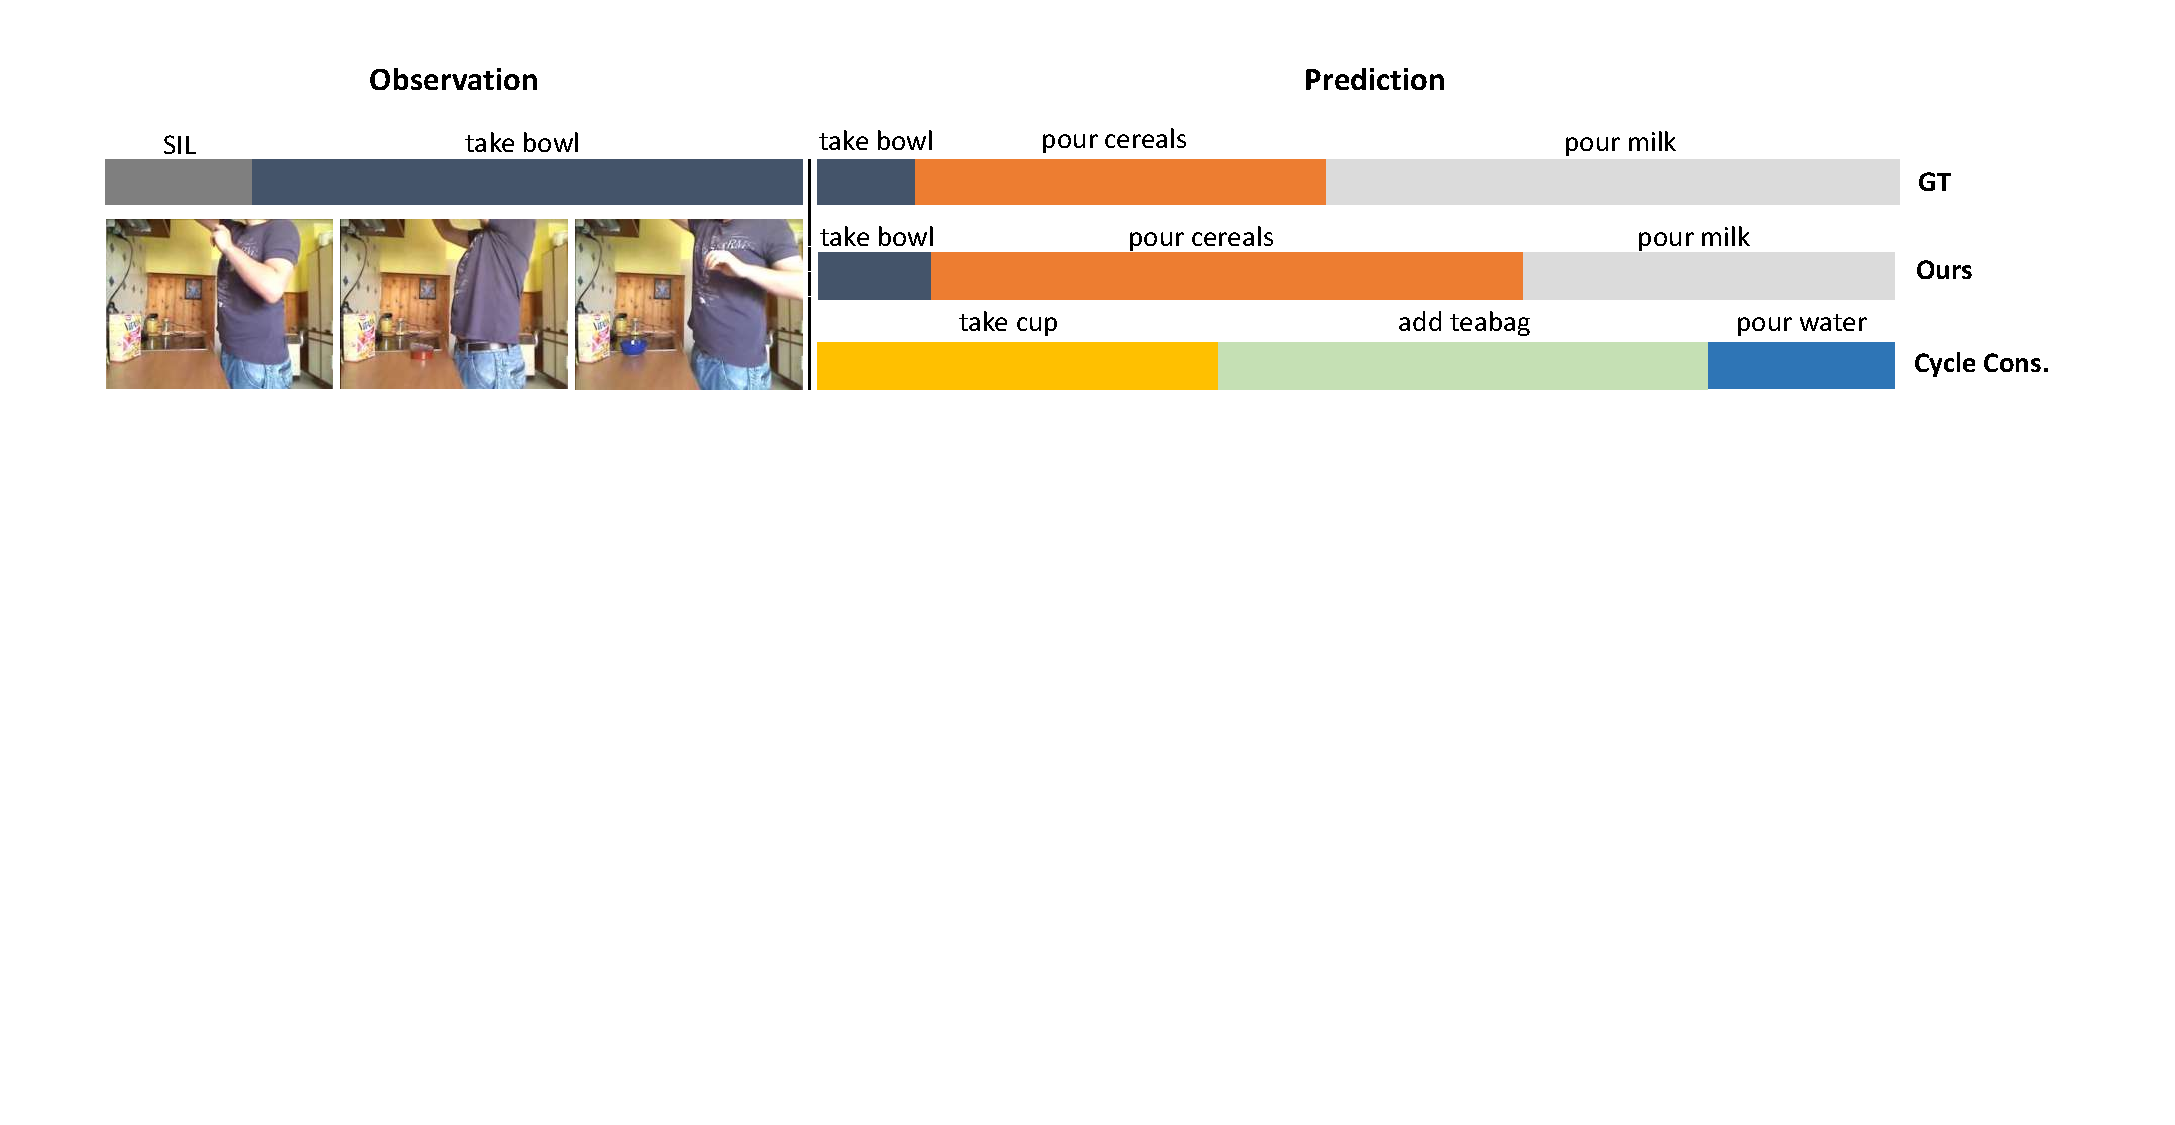
\includegraphics[width=\columnwidth]{Figures/pdf/qual_1_compressed.pdf}
    \caption{Activity: Cereal}
    \label{fig:5a}
    \end{subfigure}
    \vspace{-1mm}
    \begin{subfigure}[t]{\linewidth}
    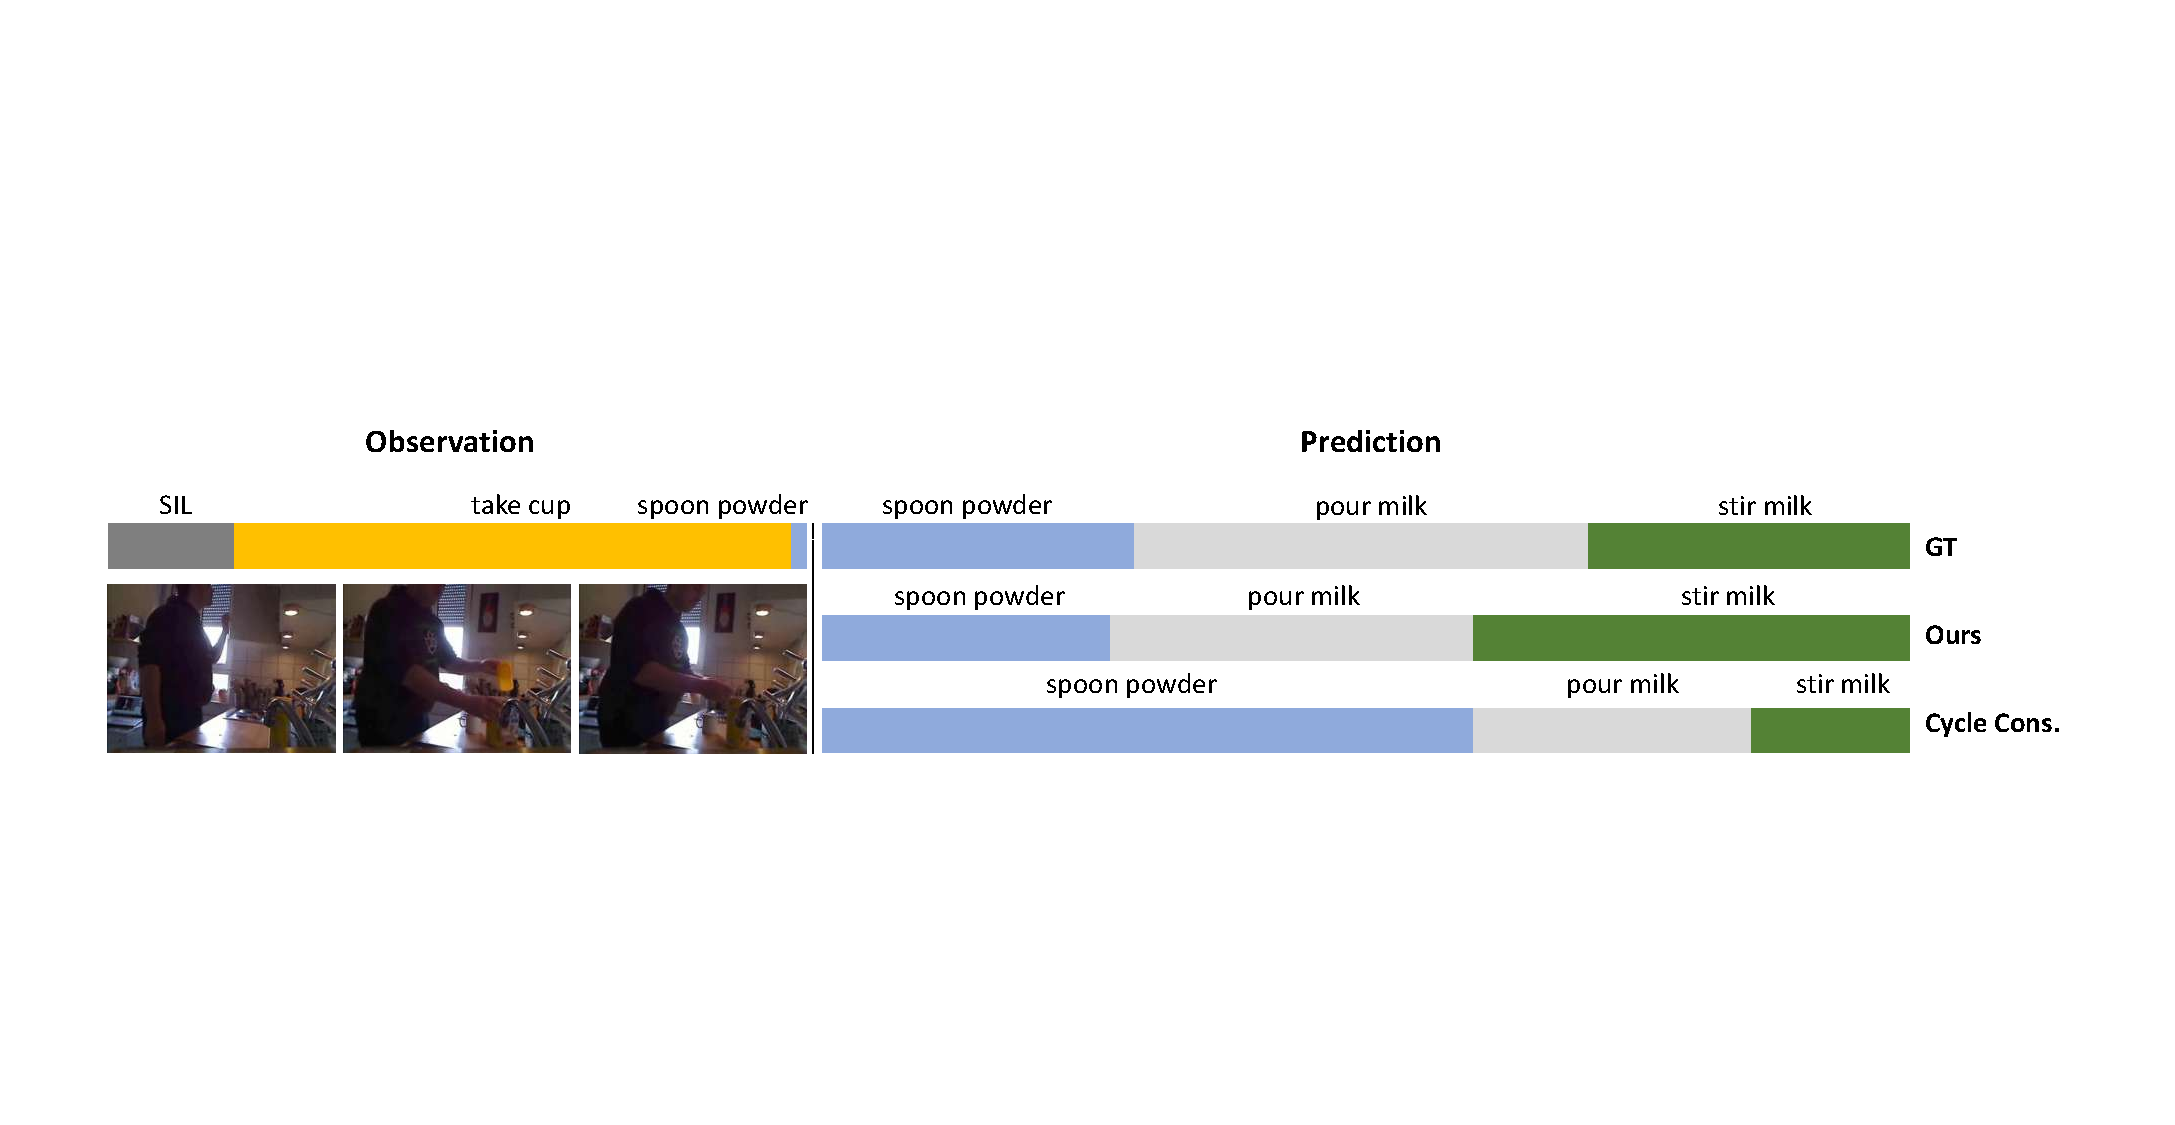
\includegraphics[width=\columnwidth]{Figures/pdf/qual_2_compressed.pdf}
    \caption{Activity: Milk}
    \label{fig:5b}
    \end{subfigure}
    \vspace{-1mm}
    \begin{subfigure}[t]{\linewidth}
    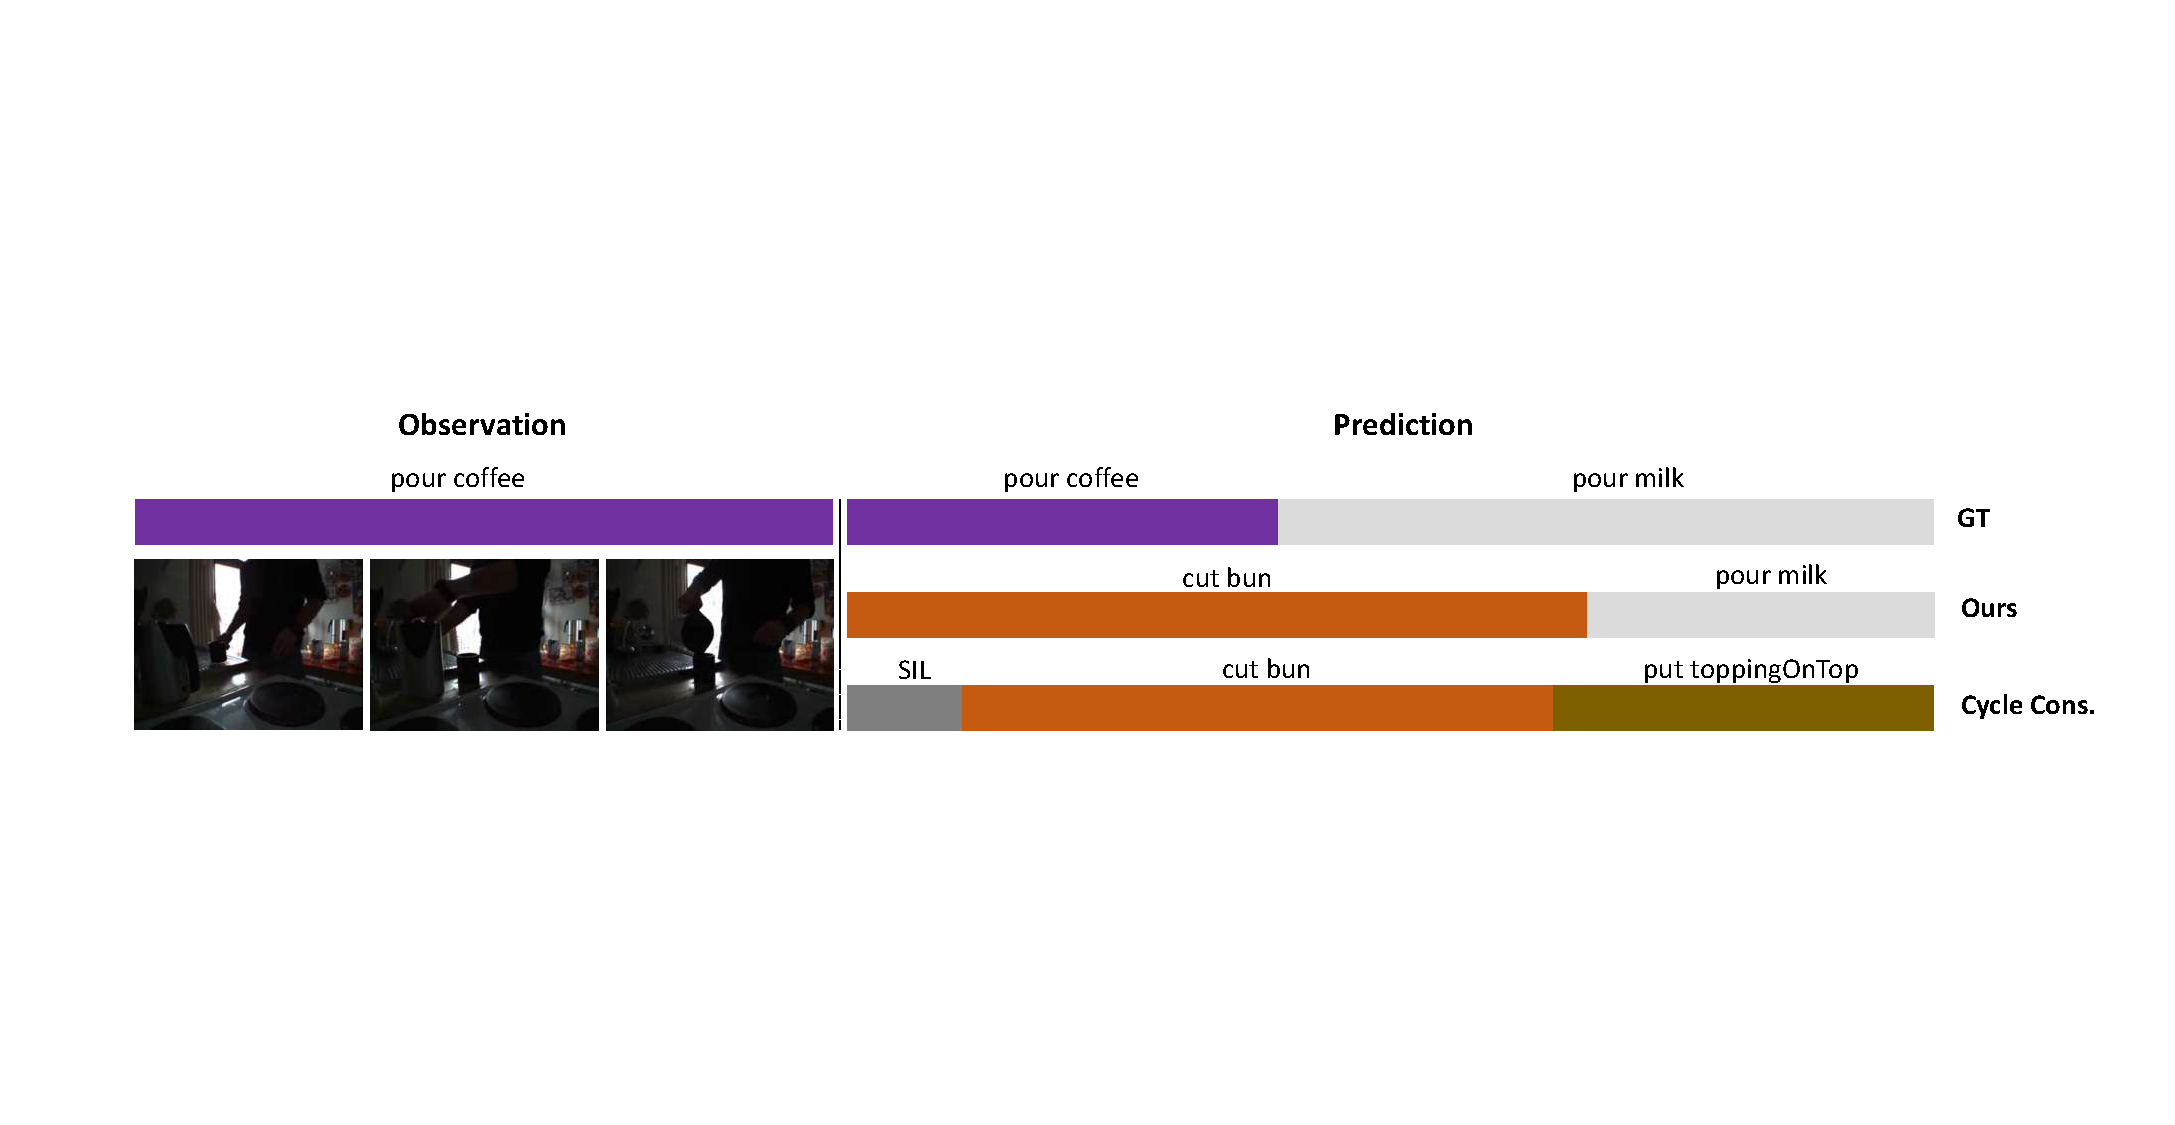
\includegraphics[width=\columnwidth]{Figures/pdf/qual_3_compressed.pdf}
    \caption{Activity: Coffee}
    \label{fig:5c}
    \end{subfigure}
\caption{\textbf{Qualitative results on Breakfast}. Each subfigure visualizes the ground-truth labels and predicted results of the \ours and the Cycle Cons.~\cite{farha2020long}. We set $ \alpha $ as 0.3 and $ \beta $ as 0.5 in this experiment. We decode action labels and durations as frame-wise action classes. Each color in the color bar indicates an action label written above.}
\vspace{-4mm}
 \label{fig:5}
\end{figure*}